\chapter{Conception et développement}
\label{ch:condev}

	\section{Architecture du logiciel}

		\subsection{Vision globale}
			
			D'un point de vue matériel, le système est séparé en deux parties: la plateforme mobile, robot sur lequel sont connectés les périphériques de capture, et le poste de contrôle, terminal de consultation des informations par l'opérateur humain. Le schéma \autoref{fig:diag_gen} expose cette architecture en détail.
			\begin{figure}[h]
			{
				\centering
				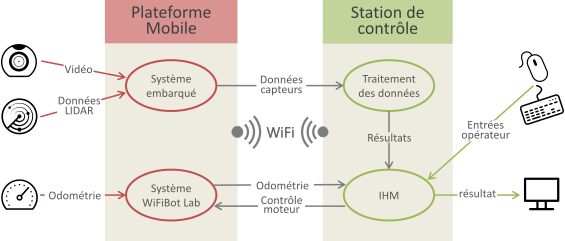
\includegraphics[width=1\textwidth]{figures/diag_general.pdf}
				\caption{Schéma de l'architecture générale du système}
				\label{fig:diag_gen}
			}
			\end{figure}
			\par
			La plateforme mobile est un \emph{WiFiBot Lab V3}\cite{wifibot}, fourni par l'INSA Centre-Val-de-Loire, dont la carte de contrôle, munie d'un processeur x86, fonctionne sous Windows XP Embedded et dispose d'un serveur connecté par WiFi à un routeur (fourni également) permettant de lui envoyer des commandes de contrôle des moteurs des roues. Dans un souci de conservation de l'existant et par simplicité de développement, nous avons choisi de contrôler les périphériques et de centraliser les transfers de données des capteurs au travers d'un Raspberry Pi 3 modèle B, qui possède une puissance de calcul raisonnable face à sa faible consommation et une carte WiFi intégré. Par ailleurs, le fait que ce micro-ordinateur fonctionne sous Linux nous permet de conserver une continuité dans le choix des technologies logicielles à utiliser.
			\par
			Le poste de contrôle, connecté au même routeur que le WifiBot, est constitué d'un micro-ordinateur disposant d'un \gls{gpu} dédié (NVIDIA K620), d'un écran et de périphériques d'entrées standard (clavier, souris), permettant d'intéragir avec l'opérateur. Au vu de la faible puissance de calcul dont dispose la plateforme mobile, le choix a été fait de centraliser les traitements lourds sur ce poste.
			\par
			Le logiciel se scinde en deux parties bien distinctes:
			\begin{description}[noitemsep]
				\item[l'Interface Homme-Machine], qui permet à l'opérateur de contrôler les mouvements de la plateforme mobile, démarrer les périphériques de capture et leurs chaînes de traitement, d'enregistrer une mission et de visionner le déroulement d'une mission enregistrée.
				\item[le réseau de traitement de données], qui permet d'exploiter les données en sortie des périphériques de capture de manière à en tirer des informations pertinentes: la cartographie des lieux visités et les objets d'intérêt qui y sont présents.
			\end{description}

		\subsection{Réseau de traitement de données}

			\change[inline]{Ajouter schéma réseau ros}
			\content[inline]{A faire}
			
		\subsection{Interface Homme-Machine}
		\label{sub:ihm}

			\change[inline]{Ajouter schéma archi ihm}
			\content[inline]{A faire}

	\section{Réalisations}
	
		\subsection{Transmission de la vidéo}
		
			La caméra Ricoh Theta S comporte une carte WiFi, ce qui permet, pour une utilisation \og normale \fg{} (avec l'application Android fournisseur) de s'y connecter avec un téléphone fonctionnant sous Android, afin d'y transférer les données de la caméra. Ces données peuvent prendre la forme de photos ou de vidéos, préalablement enregistrées sur la mémoire interne de la caméra et donc récupérées en différé, ou d'un mode spécial, nommé \emph{live}, qui permet de transmettre un flux vidéo continu correspondant à la capture des objectifs de la caméra en temps réel. Ce mode permet de transmettre un aperçu au téléphone avant de prendre une photo, uniquement supporté par l'application Android du fabricant. Devant la demande croissante du public d'utiliser ce mode de \og livestream \fg{}, les développeurs ont choisi de le rendre disponible sur pc, au travers d'un pilote matériel permettant aux OS \emph{Windows} et \emph{Mac OS} de considérer la caméra, alors branchée à l'ordinateur par \gls{usb}, comme une webcam, permettant ainsi la plupart des programmes d'exploiter ce flux vidéo. Ce pilote se charge de communiquer avec le bon protocole les commandes utilisateurs à la caméra et de transformer le flux vidéo dans un format exploitable. Après analyse du pilote windows, il a été découvert (car non exprimé dans la documentation du produit) qu'il utilise la bibliothèque \emph{libUVC}, et donc que la communication avec la caméra est effectuée au travers du protocole \gls{uvc}. La caméra étant sur la plateforme mobile disposant d'un \emph{Raspberry Pi 3b}, il a été développé un noeud \gls{ros} permettant de lui envoyer des commandes, d'acquérir le flux vidéo direct et de l'envoyer sur le poste de contrôle.
			\par
			Une problématique arrivée rapidement est celle de la transmission sur le WiFi.
			La Raspberry Pi dispose d'une carte WiFi qui ne supporte que la norme 802.11g, et ne peut donc transférer des données qu'au débit réel maximal de 25 Mb/s.
			Après une analyse de paquet en cas réel, la bande passante disponible pour le flux vidéo n'est que de 17,6 Mb/s, soit 2,2 Mo/s.
			Une image \gls{jpeg} en sortie de la caméra pèse en moyenne 400ko, et la caméra opère à 15 images/s, ce qui nécessite un débit de 6M/s.
			La Raspberri Pi dispose d'un \gls{gpu} \emph{VideoCore IV}\cite{videocore}, servant en priorité à encoder et décoder des vidéos (par exemple, pour lire un flux vidéo en haute qualité depuis internet).
			Il est donc possible d'utiliser la bibliothèque \emph{OpenMAX} pour encoder une vidéo, qui devrait donc peser moins qu'une séquence d'images décorrélées.
			Cependant, après de nombreux éssais d'envoi de flux converti (au format h264, le format le plus optimisé pour cette puce graphique), il s'est avéré que l'encodage entraîne un surplus de traitement au niveau du processeur de la Raspberry, qui entraîne l'introduction d'une latence importante entre la capture d'une image et sa visualisation sur le poste opérateur.
			Il a donc été décidé de réduire la vitesse du flux de la caméra à 5 images/s, afin de ne nécessiter que 2Mo/s de bande passante.
			%1 jpeg 1280x768 = 400ko
			% 5 fps = 2000ko/s
			%15 fps = 6000ko/s
			%wifi        54   mb/s | 6.75  mo/s
			%            25   mb/s | 3.125 mo/s
			%benchmarks: 17.6 mb/s | 2.2   mo/s
			\par
			Les images sont donc extraites des paquets \gls{usb} et envoyées au poste de contrôle encapsulées dans un protocole simple et efficace pour la transmission de données unidirectionnelle en temps réel, dont l'unité de donnée (\gls{pdu}) est la suivante:

			\begin{center}
				\scriptsize
				\begin{tabular}[h]{|c|c||c|}
					\toprule
					\multicolumn{2}{|c||}{entête (24 octets)} & charge utile (variable) \\
					\midrule
					Identifiant protocole (8 octets) & taille image (16 octets) & données (variable)\\
					\bottomrule
				\end{tabular}
			\end{center}

			Ces trames sont encapsulées dans des trames \gls{tcp} pour laisser le système s'occupper de la fragmentation et de l'ordonnacement, ce qui simplifie le traitement du côté réception et du côté traitement des données (pas de mise en file d'attente).
			
		\subsection{Transformation vidéo}
		\label{sub:transfo}
		
			En sortie de la caméra, l'image correspond aux photos prises par les deux objectifs, chacun ayant un angle de prise de vue de $190^{\circ}$, horizontalement et verticalement, et chacun étant de type \gls{fisheye} circulaire. Un exemple d'image non traitée est représenté \autoref{fig:rawcapture}. Le fait de disposer de deux photos \gls{fisheye} qui couvrent l'ensemble du point de vue à la position de la caméra s'appelle couramment \emph{Dual Fisheye}. On peut parler de représentation sphérique d'un point de vue, l'angle de champ étant de $360^{\circ}\times180^{\circ}$. Les caractéristiques spatiales visibles observent un niveau de déformation proportionnel à leur éloignement du centre de l'objectif. À défaut de traitement, la détection et la classification des objects contenus dans la scène présentent des imprécisions qui rendent de tels résultats inexploitables.
			\begin{figure}[h]
			{
				\centering
				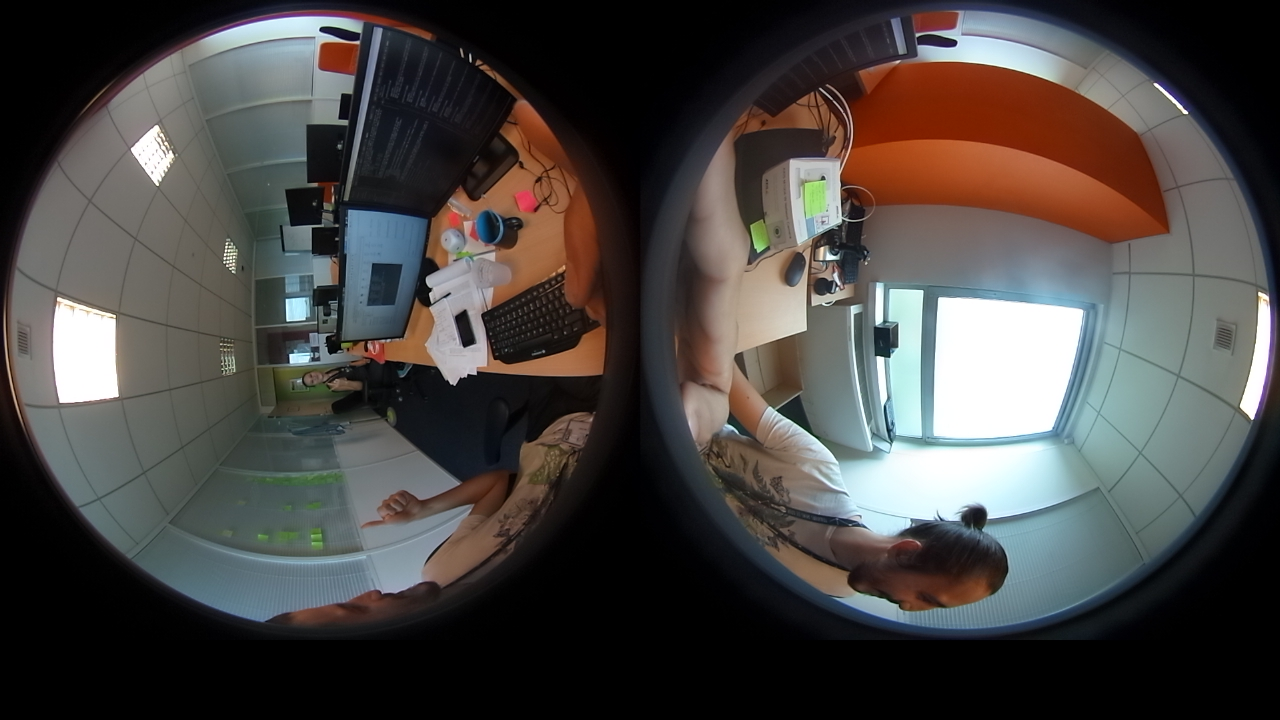
\includegraphics[width=1\textwidth]{figures/capture.jpg}
				\caption{Image non traitée capturée en sortie de la caméra}
				\label{fig:rawcapture}
			}
			\end{figure}
			\par
			Comme évoqué dans la section précédente, le pilote fourni par le fabricant transforme cette image en appliquant une projection spatiale sur chacun de ses pixels de manière à obtenir une couverture complète du point de vue en projection équirectangulaire. Cette méthode permet de voir l'intégralité de la surface d'une sphère sur un plan. Les figures suivantes visent à illustrer cette opération.
			\par
			On considère la scène \autoref{fig:cage}, où notre point de vue correspond à la sphère rouge. Notre scène comporte donc une cage dont les faces ont des couleurs différentes et des numéros permettant de mettre les caractéristiques spatiales en valeur.
			\begin{figure}[h]
			{
				\centering
				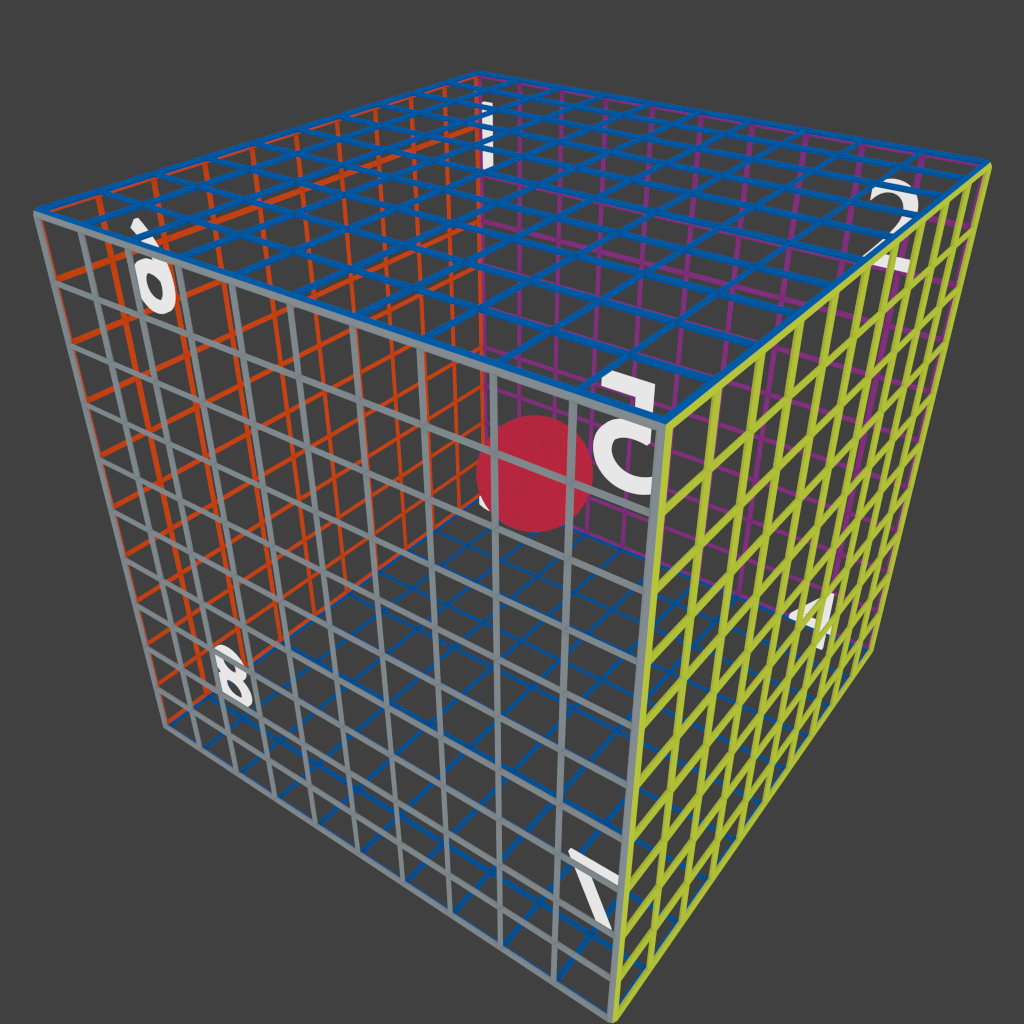
\includegraphics[width=0.6\textwidth]{figures/cage.png}
				\caption{Scène d'exemple vue de l'extérieur}
				\label{fig:cage}
			}
			\end{figure}
			\par
			On se place maintenant à l'intérieur, en direction du côté violet (face du fond), et on prend deux photographies -- respectivement vers l'avant et vers l'arrière -- à l'aide d'un objectif \gls{fisheye} avec un angle de champ de $180^{\circ}$. On obtient alors l'ensemble du point de vue sous la forme de deux disques comme vus en \autoref{fig:dualfish}.
			\begin{figure}[H]
			{
				\centering
				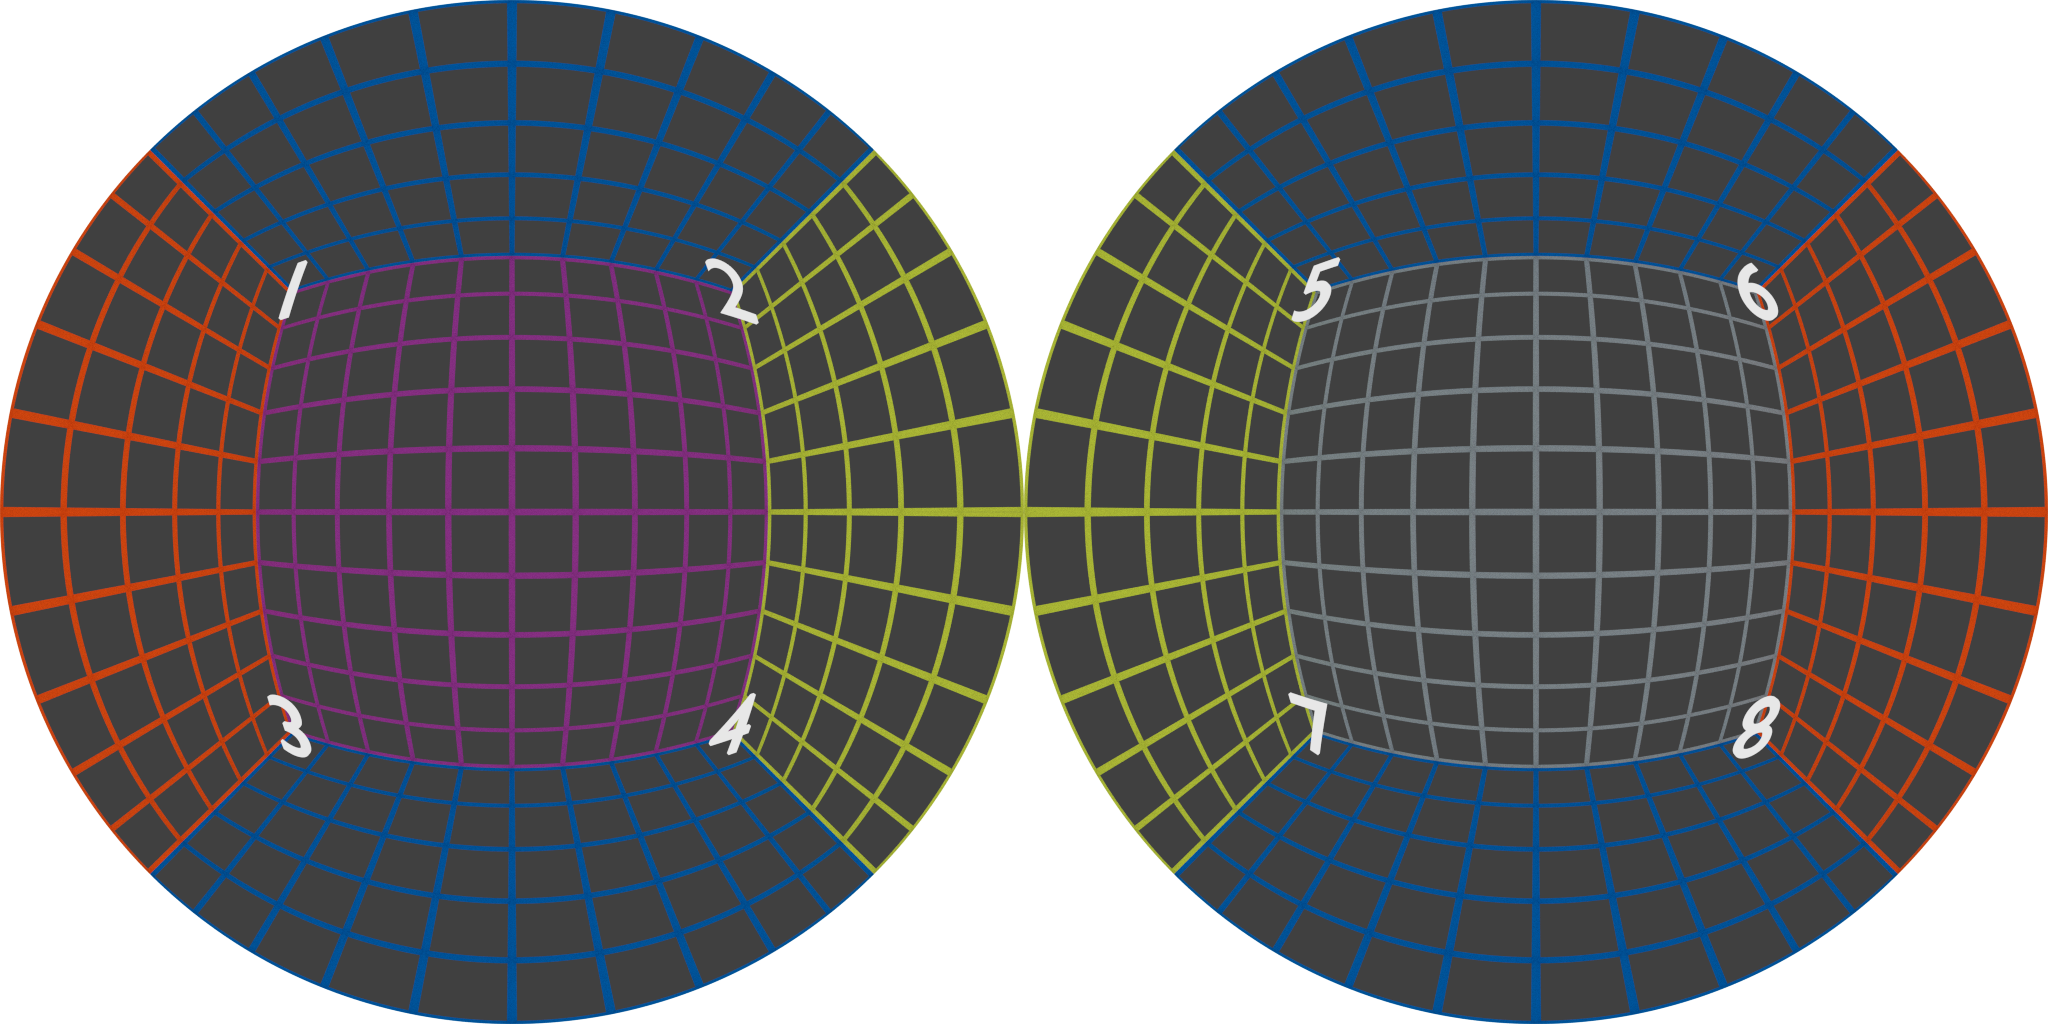
\includegraphics[width=1\textwidth]{figures/dfish.png}
				\caption{Vue sphérique \og dual fisheye \fg{}}
				\label{fig:dualfish}
			}
			\end{figure}
			\par
			On crée alors un rectangle où chaque pixel trouve un correspondant dans ces disques, et on obtient une projection equirectangulaire de l'espace sphérique d'origine. (\autoref{fig:equirect}).
			\begin{figure}[H]
			{
				\centering
				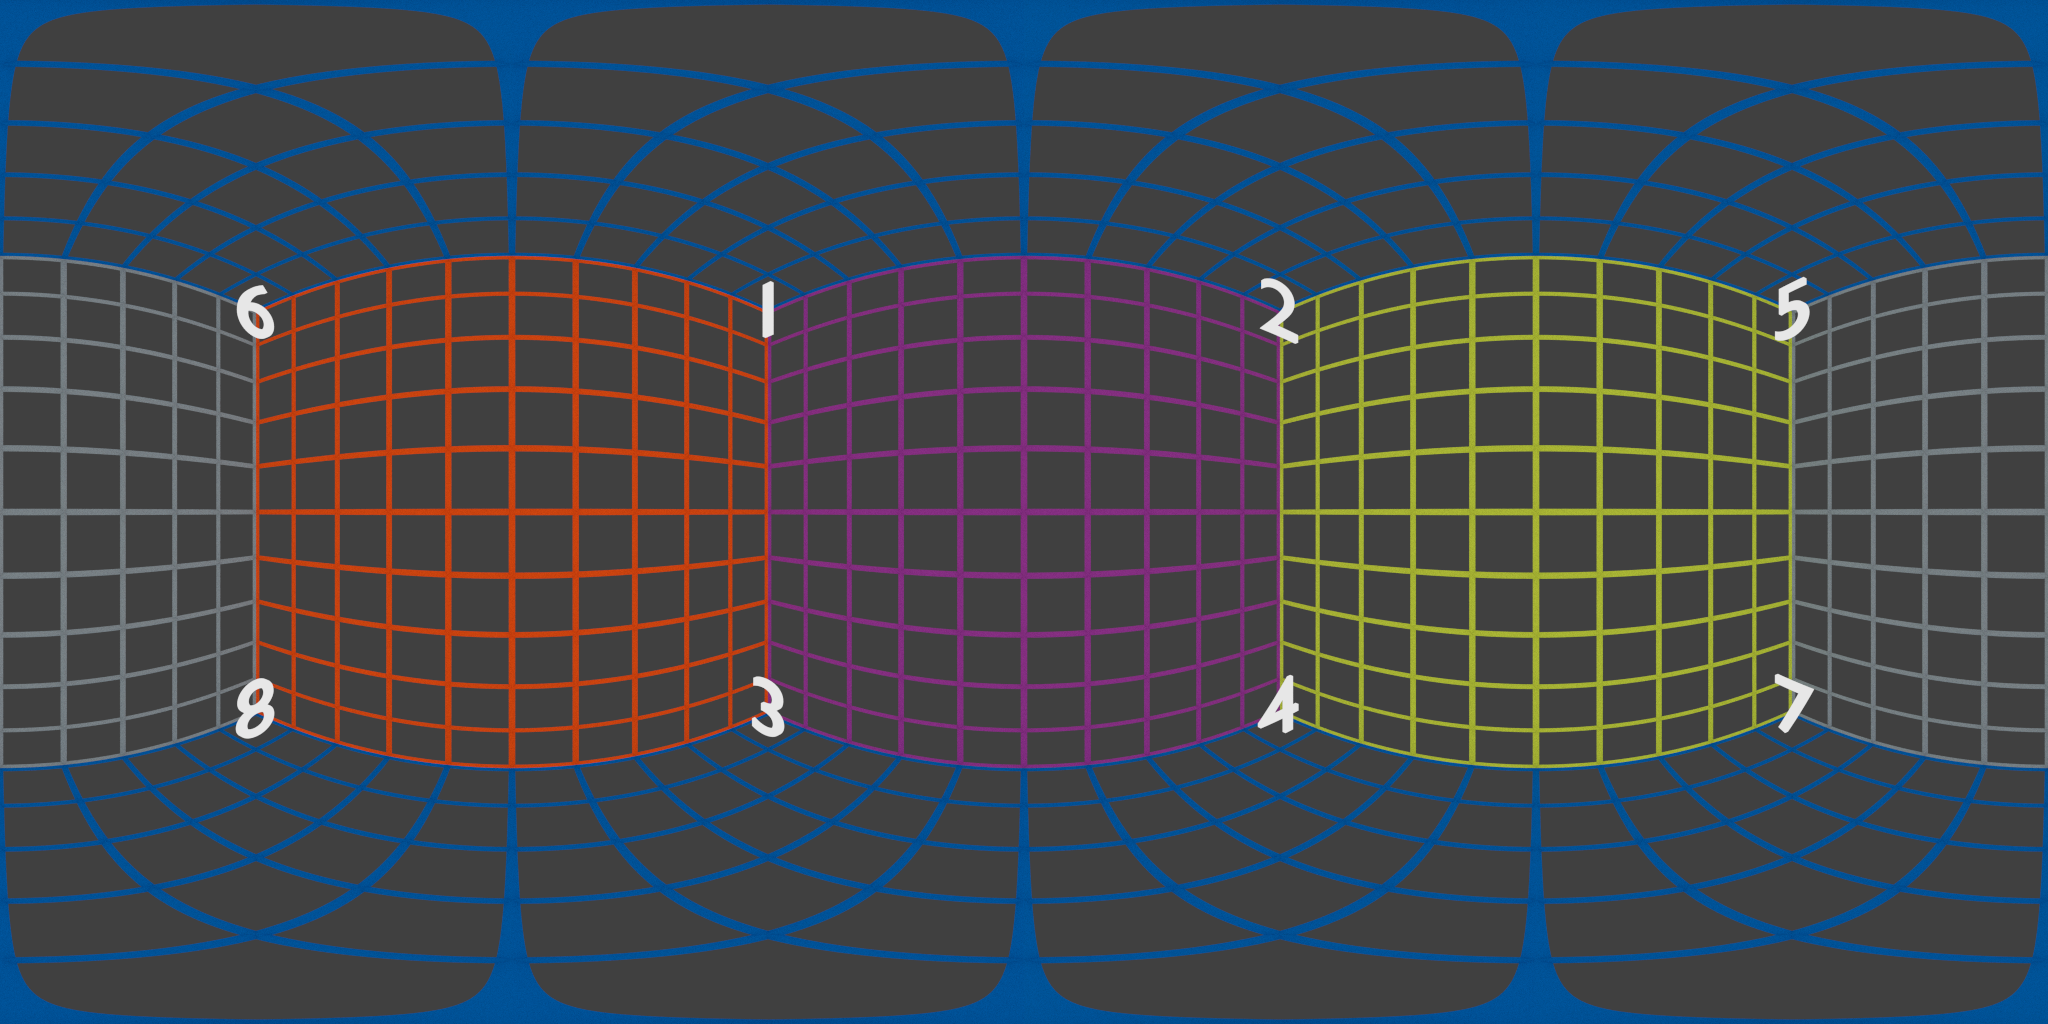
\includegraphics[width=1\textwidth]{figures/equirect.png}
				\caption{Projection equirectangulaire}
				\label{fig:equirect}
			}
			\end{figure}
			Bien qu'elles soient toujours déformées, les faces orange et verte deviennent assez linéaires pour présenter des caractéristiques spatiales détectables. On opère alors la détection sur cette image.
			\par
			L'opération mathématique correspondante revient à effectuer trois projections spatiales successives pour chaque pixel, ce qui justifie l'emploi du processeur graphique pour sa haute parallélisation des calculs.
			\par
			La première projection revient à retrouver les coordonnées sphériques réelles de l'objectif de la caméra à partir des coordonnées polaires des disques \emph{fisheye}. En effet, l'objectif est vu comme une hémisphère parfaite de rayon 1, afin de simplifier les calculs. Notons toutefois que l'objectif réel n'est pas une hémisphère parfaite, ce qui introduit l'utilisation de la distance focale dans les calculs afin de minimiser les déformations induites par cette approximation.
			\begin{figure}[htb]
				\centering
				\begin{minipage}{.5\textwidth}
					\centering
					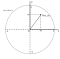
\includegraphics[width=0.95\linewidth]{figures/polar.pdf}
					\captionof{figure}{Coordonnées \newline cartésiennes sur image fisheye}
					\label{fig:pcart1}
				\end{minipage}%
				\begin{minipage}{.5\textwidth}
					\centering
					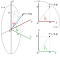
\includegraphics[width=0.95\linewidth]{figures/spherical.pdf}
					\captionof{figure}{Coordonnées sphériques (lentille de la caméra)}
					\label{fig:psph}
				\end{minipage}
			\end{figure}
			\par
			Le repère $(O,\vec{x},\vec{y})$ de la \autoref{fig:pcart1}, correspond à un disque de la photographie \emph{dual fisheye}, $O$ étant son centre.
			Le repère $(O,\vec{x},\vec{y},\vec{z})$ de la \autoref{fig:psph} correspond à l'espace réel de l'objectif de la caméra, avec $O'$ qui correspond au foyer focal du système optique.
			La correspondance entre ces repères est définie comme suit:
			\begin{center}
				$\forall P(x_{0},y_{0}) \in (O,\vec{x},\vec{y}), \exists P'(r,\theta,\phi) \in (O,\vec{x},\vec{y},\vec{z})$ avec $(x_{0},y_{0}) \in [-1;1]^2$ tel que: \newline
				$P'(x_{1},y_{1},z_{1}): \left\{
				\begin{array}{ll}
				\theta = \cos^{-1}{\left(\frac{x_{0}}{\sqrt{x_{0}^2+y_{0}^2}}\right)} \\
				\phi = \sin^{-1}{\left(\sqrt{x_{0}^2+y_{0}^2}\right)} \\
				r = 1
				\end{array}
				\right.\ $
			\end{center}
			L'étape suivante est d'utiliser les coordonnées cartésiennes de $P'$ afin d'obtenir la position (latitude, longitude) du point sur la sphère de l'espace de l'objectif de la caméra:
			\begin{center}
				$P'(x_{1},y_{1},z_{1}): \left\{
				\begin{array}{ll}
				x_{1} = r \sin \phi \cos \theta \\
				y_{1} = r \sin \phi \sin \theta \\
				z_{1} = r \cos \theta
				\end{array}
				\right.\ $ \newline \newline
				$ latitude = \tan^{-1}_{2}\left(y_{1}, x_{1}\right) $ \newline
				$ longitude = \tan^{-1}_{2}\left(z_{1}, \sqrt{x_{1}^2+y_{1}^2}\right) $ \newline
			\end{center}
			Finalement, on projette ces coordonnées depuis le plan sphérique sur un plan equirectangulaire:
			\begin{center}
				$P''(x_{2},y_{2}): \left\{
				\begin{array}{ll}
				x_{2} = \frac{longitude}{\pi} \\
				y_{2} = \frac{2 \times latitude}{\pi}
				\end{array}
				\right.\ $
			\end{center}
			
			\begin{figure}[H]
				\centering
				\begin{minipage}{.5\textwidth}
					\centering
					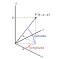
\includegraphics[width=0.95\linewidth]{figures/cartesian.pdf}
					\captionof{figure}{Latitude - longitude}
					\label{fig:platlong}
				\end{minipage}%
				\begin{minipage}{.5\textwidth}
					\centering
					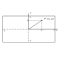
\includegraphics[width=0.95\linewidth]{figures/cart2.pdf}
					\captionof{figure}{Position equirectangulaire}
					\label{fig:pequirect}
				\end{minipage}
			\end{figure}
			\par

		\subsection{Détection et Classification}
		
			Afin d'intégrer le module de détection et classification dans le système \gls{ros},
			\info[inline]{WIP}
			\par
			
			Comme vu en partie \todoref, les réseaux de neurones convolutifs prennent toujours une entrée de taille fixe.
			Dans le cas de \emph{YOLO}, l'entrée doit être une image RGB de dimensions $ 418px \times 418px $ (ratio $1:1$), alors que les images en sortie de la caméra sont de dimension $ 1280px \times 720px$ (ratio $16:9$).
			Le redimensionnement de l'image introduit alors des déformations importantes qui aggravent celles déjà induites par la projection equirectangulaire.
			Les résultats d'une détection s'en retrouvent donc dégradés (\autoref{fig:pred_b}).
			\begin{figure}[H]
			{
				\centering
				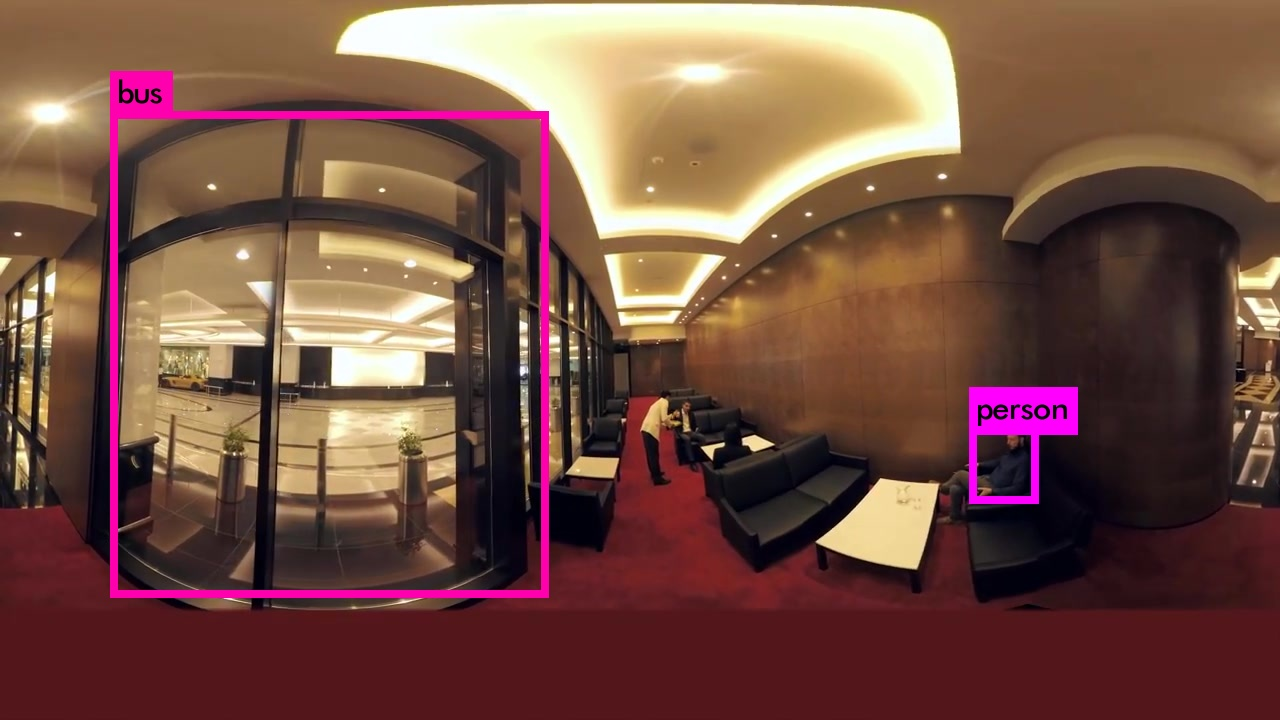
\includegraphics[width=.8\textwidth]{figures/predictions_bad.jpg}
				\caption{Détection sur image $360^{\circ}$}
				\label{fig:pred_b}
			}
			\end{figure}
			
			La solution adoptée consiste à fragmenter l'image en plusieurs parties afin de minimiser ces déformations. Après quelques tests\footnote{Les résultats des tests et benchmarks furent pour la plupart subjectifs, car il n'existe pas encore de bases de données d'images $360^{\circ}$ annotées.}, il s'est avéré que la méthode la plus optimale en matière de précision des détections fût de couper l'image en trois parties (en vert sur la \autoref{fig:pred_c}) et d'en ignorer 20\% (en rouge) jugés trop déformés.
			
			\begin{figure}[H]
			{
				\centering
				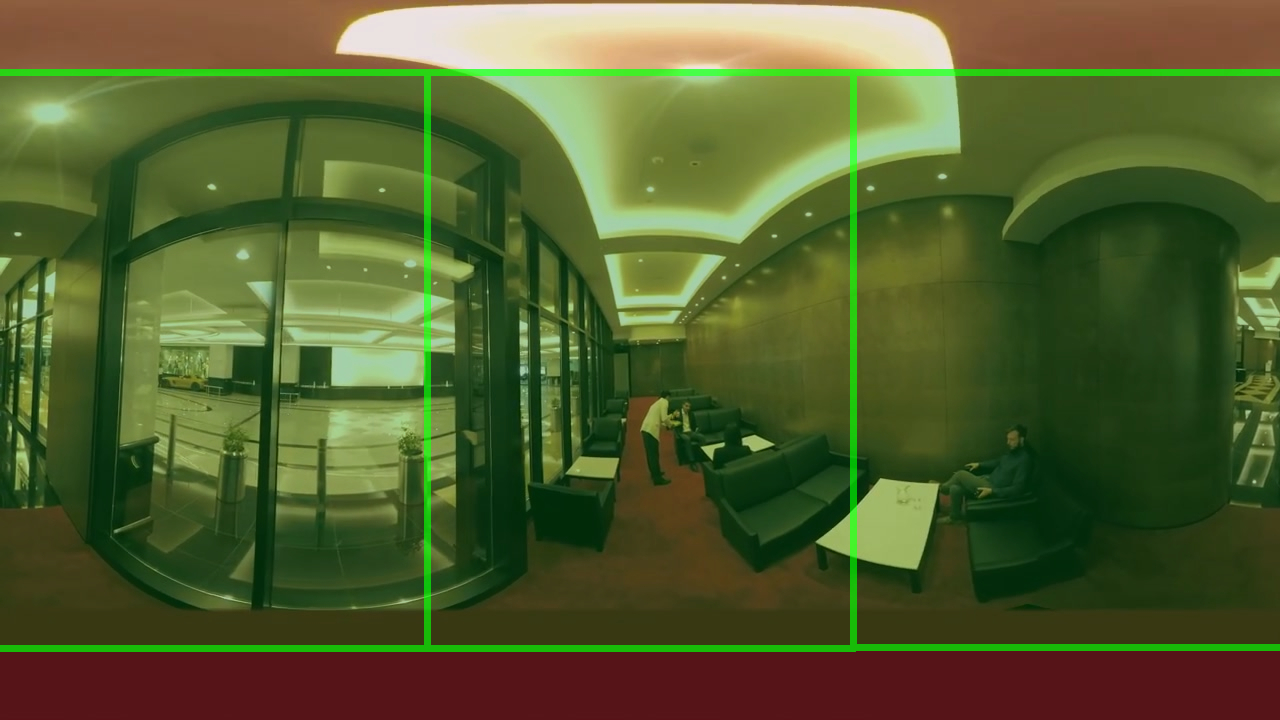
\includegraphics[width=.8\textwidth]{figures/predictions_cut.jpg}
				\caption{Fragmentation d'une image en trois parties}
				\label{fig:pred_c}
			}
			\end{figure}
			\begin{figure}[H]
			{
				\centering
				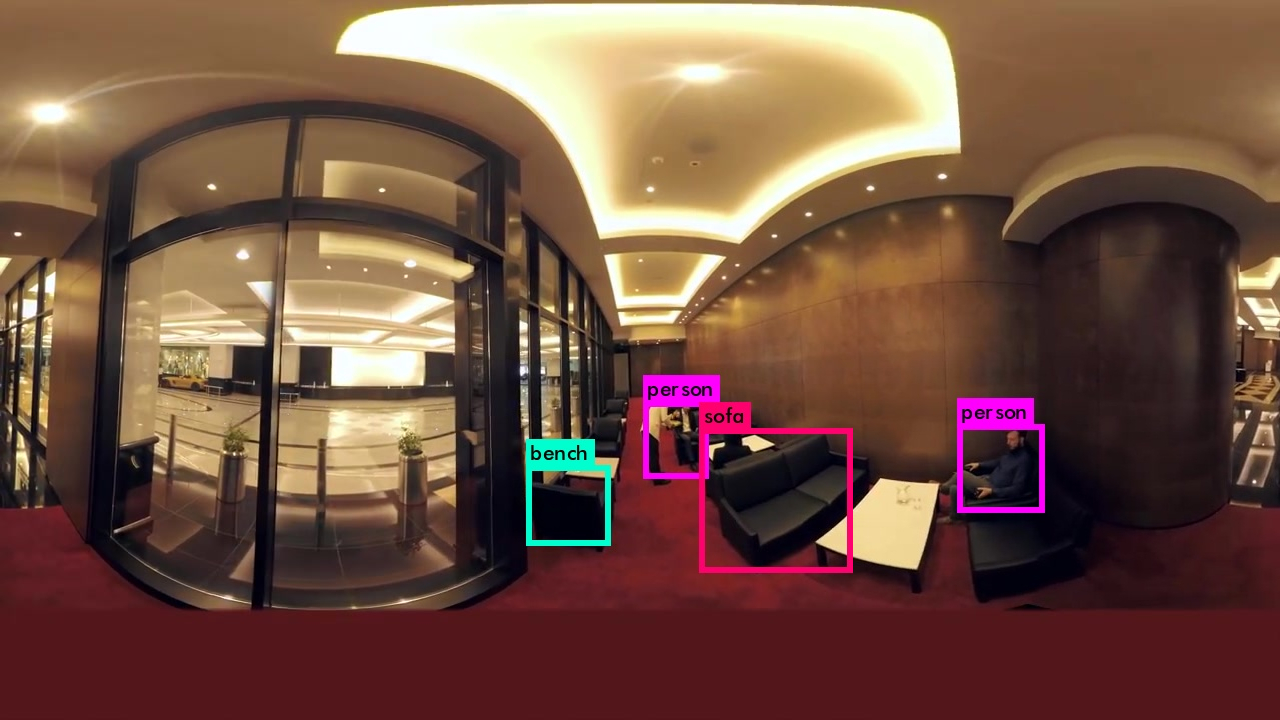
\includegraphics[width=.8\textwidth]{figures/predictions_f.jpg}
				\caption{Détection sur image fragmentée.}
				\label{fig:pred_f}
			}
			\end{figure}
			
			Bien que la qualité des détections soit devenue subjectivement acceptable (voir \autoref{fig:pred_f}), la vitesse d'opération s'en trouve amoindrie, car ce traitement multiplie par trois les opérations à effectuer pour chaque image de la caméra.
			Après consultation de M. Daumand, il a été décidé de développer trois modes d'utilisation du module de détection: un mode simple, qui traite l'image en entier, un mode \og divisé \fg{}, qui permet d'utiliser la méthode précedemment définie
			, et un mode \og fragmenté \fg{}, qui n'opère la détection que sur la partie de l'image que l'utilisateur est en train de visionner.
			
		\subsection{Présentation vidéo et incrustation}
		
		Dans les disciplines de détection et de classification, la présentation des résultats à un utilisateur se fait communément en encadrant les objets détectés avec des couleurs relatives à leurs classes (voir \autoref{fig:pred_f}) sur l'image d'origine. Cette methode simple induit dans notre cas une déformation des annotations lors de la visualisation du flux vidéo et réduit significativement l'expérience utilisateur\footnote{Une fois projetées sur une sphère, les annotations mettent en valeur la forme de projection et rendent l'image subjectivement "plate", empéchant ainsi toute forme d'immersion de l'utilisateur.} (\autoref{fig:pannot}).
		\begin{figure}[H]
		{
			\centering
			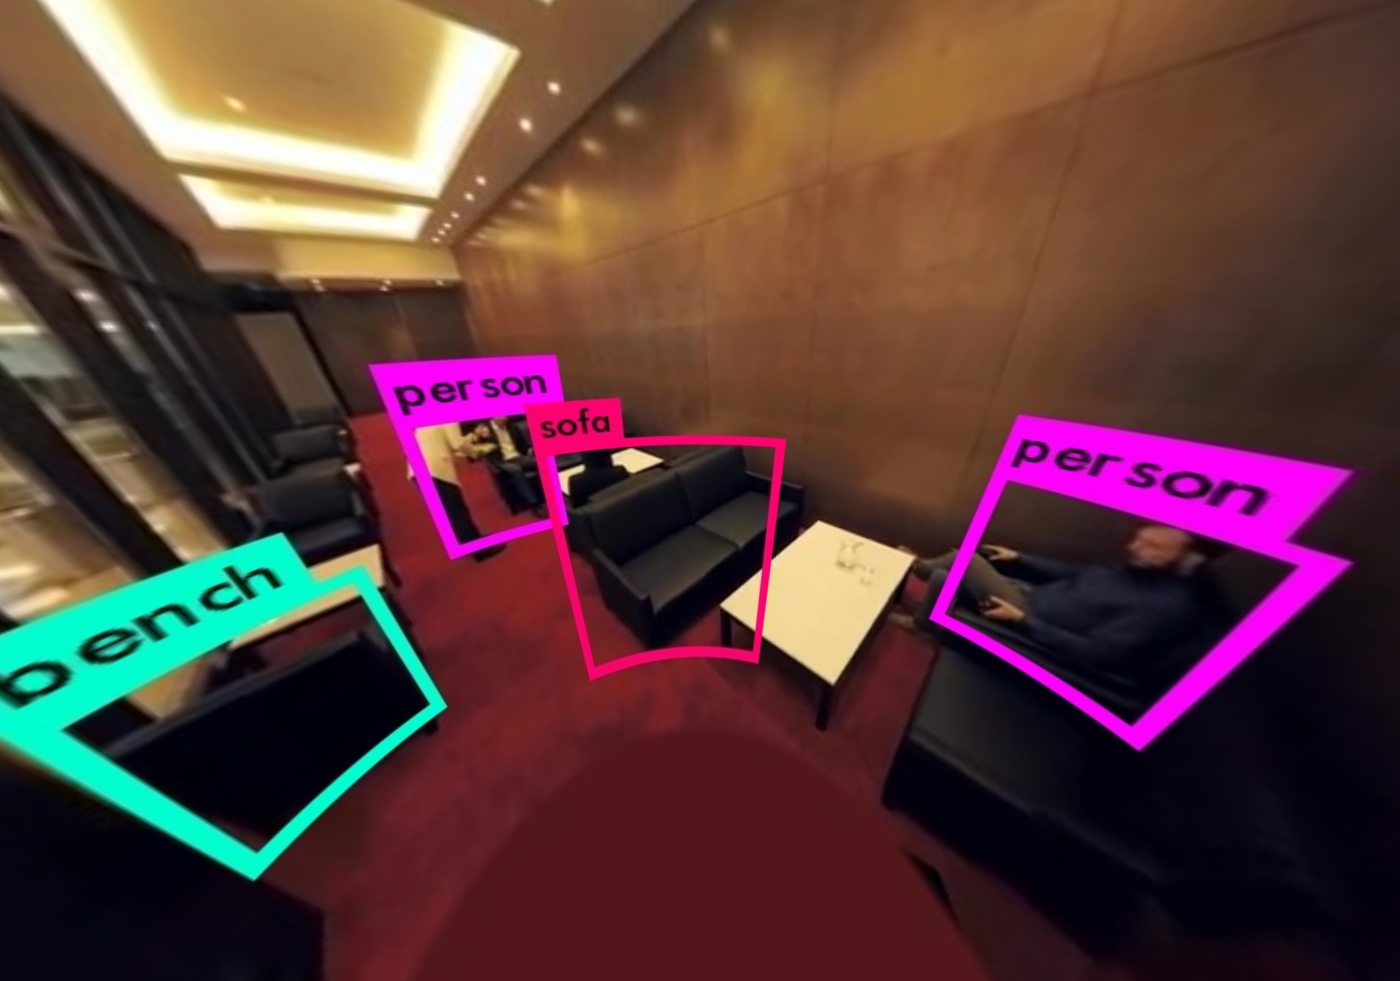
\includegraphics[width=.8\textwidth]{figures/pannot.png}
			\caption{Déformation des annotations}
			\label{fig:pannot}
		}
		\end{figure}
		Au lieu d'être incrustés directement dans l'image, les résultats sont stockés dans une structure de données comportant:
		\begin{itemize}[noitemsep]
			\item Position centrale dans l'image (en coordonnées sphériques)
			\item Largeur et hauteur dans l'image
			\item Position centrale dans l'espace\footnote{\label{ft_calc} Calculé ultérieurement} (en coordonnées cartésiennes)
			\item Largeur et hauteur dans l'espace\textsuperscript{\ref{ft_calc}}
			\item Classe
			\item Score de détection ($ 0 < score < 1 $)
		\end{itemize}
		Il est alors possible d'utiliser ces données pour des traitements ultérieurs.
		\par
		
		
		L'interface présentée en partie \ref{sub:ihm} s'occupe
		\begin{figure}[H]
			\centering
			\begin{minipage}{.5\textwidth}
				\centering
				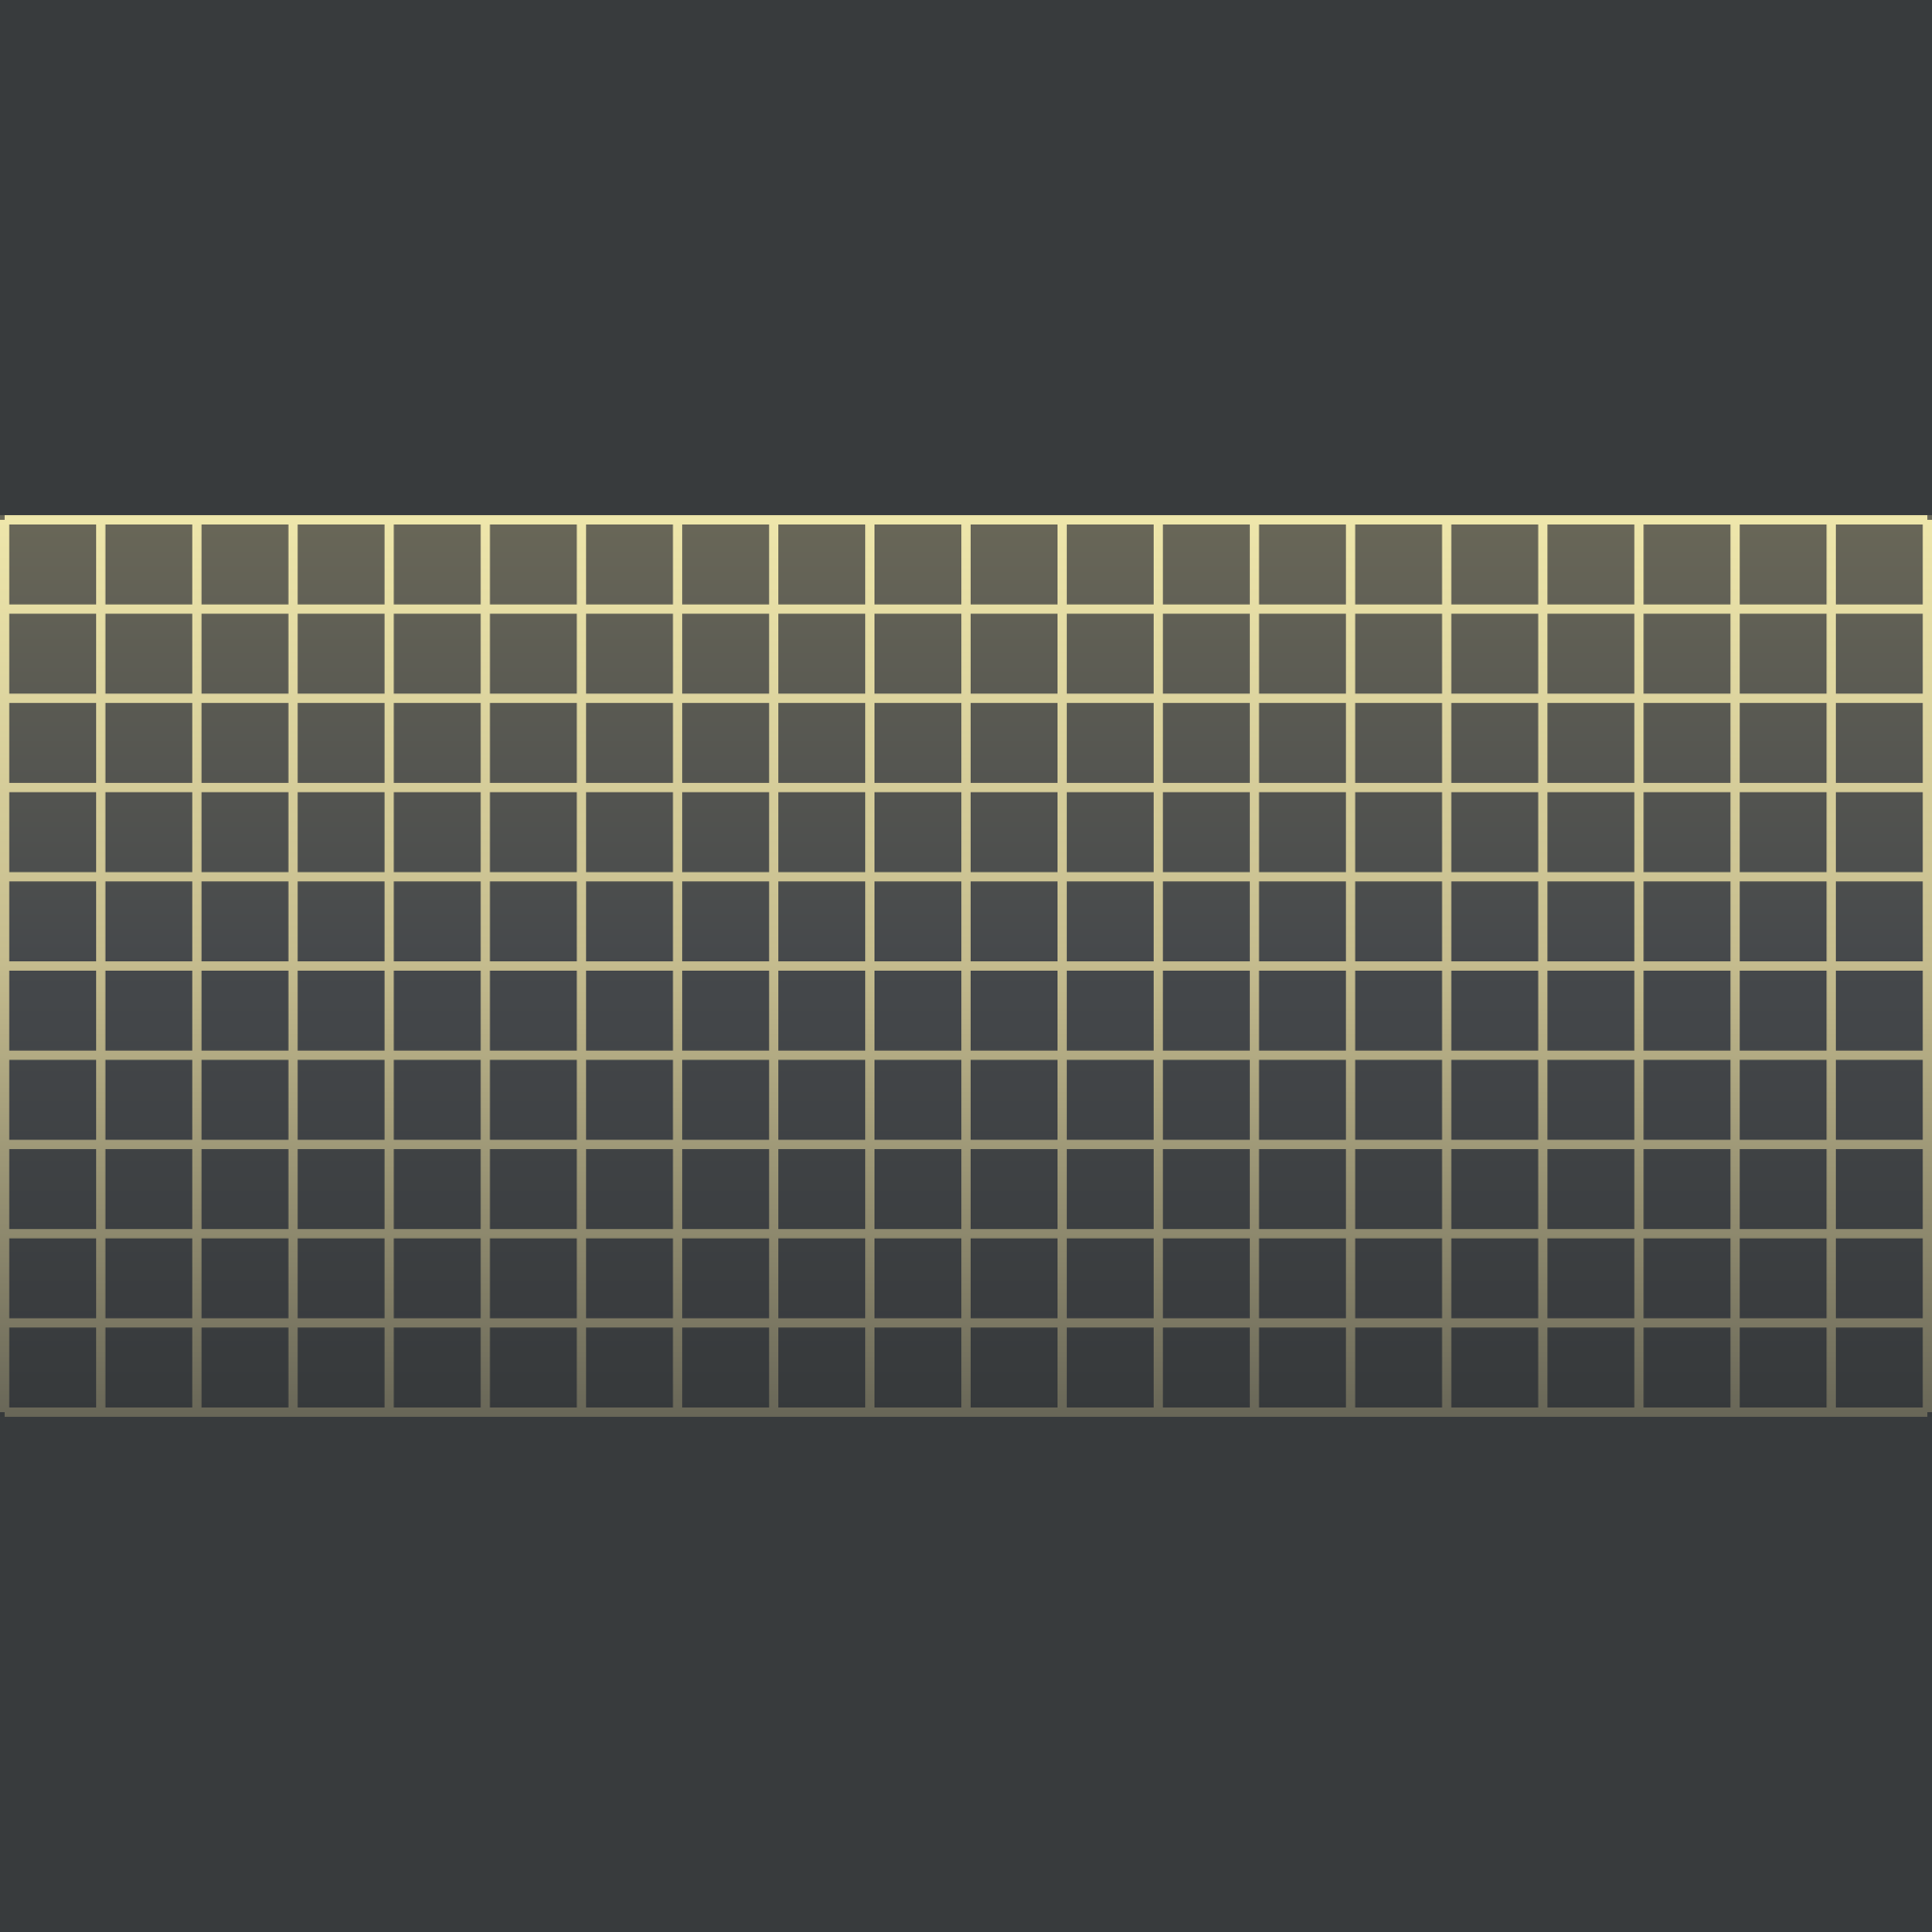
\includegraphics[width=0.95\linewidth]{figures/def0.png}
				\captionof{figure}{Image equirectangulaire}
				\label{fig:def0}
			\end{minipage}%
			\begin{minipage}{.5\textwidth}
				\centering
				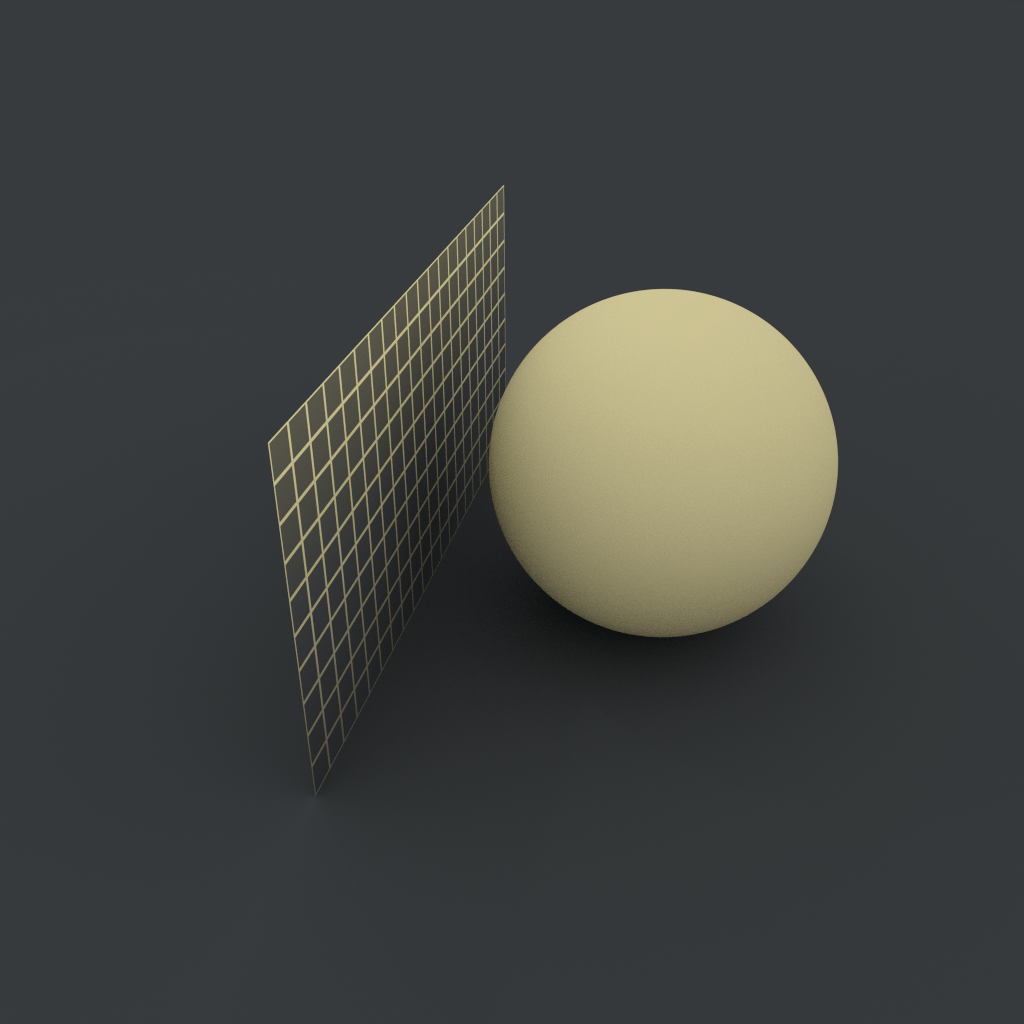
\includegraphics[width=0.95\linewidth]{figures/def1.png}
				\captionof{figure}{Texture mapping }
				\label{fig:def1}
			\end{minipage}
			
			\vspace{0.5cm}
			
			\begin{minipage}{.5\textwidth}
				\centering
				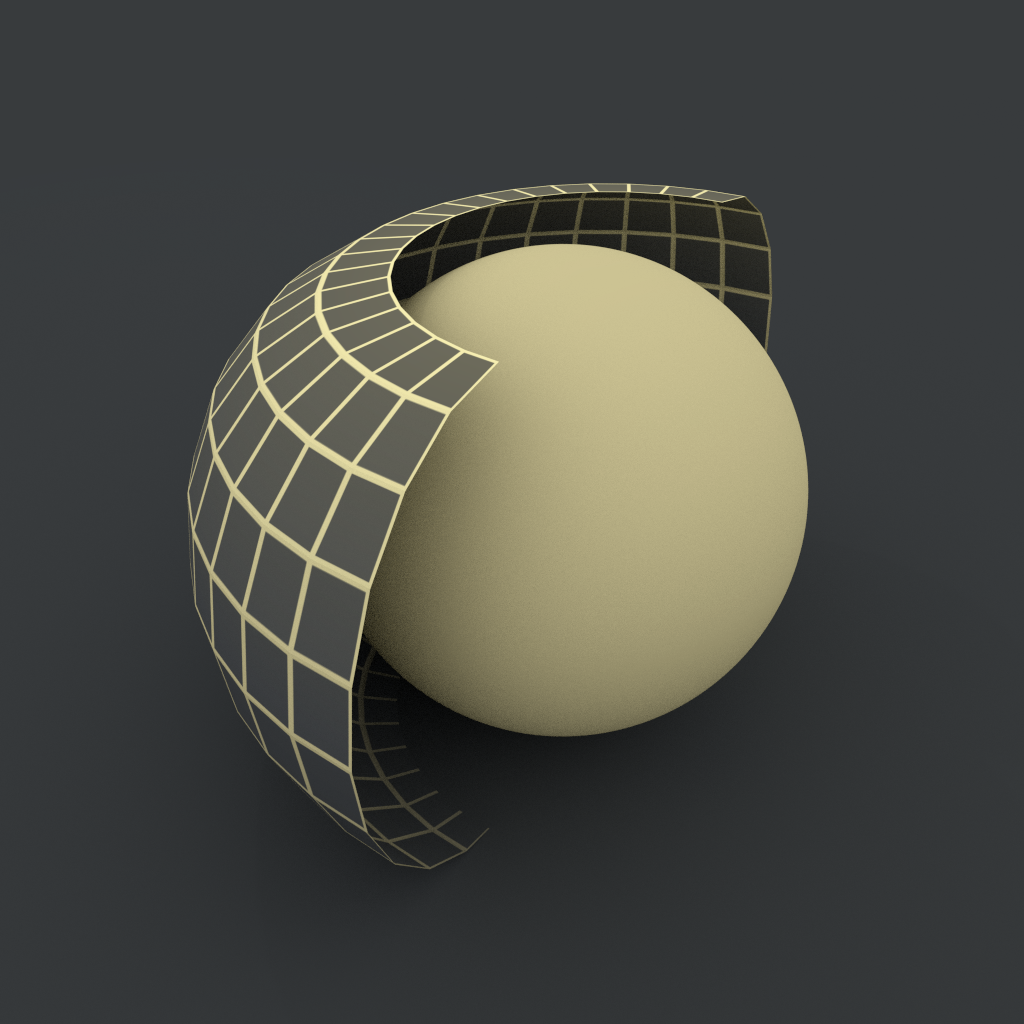
\includegraphics[width=0.95\linewidth]{figures/def2.png}
				\captionof{figure}{Déformation}
				\label{fig:def2}
			\end{minipage}%
			\begin{minipage}{.5\textwidth}
				\centering
				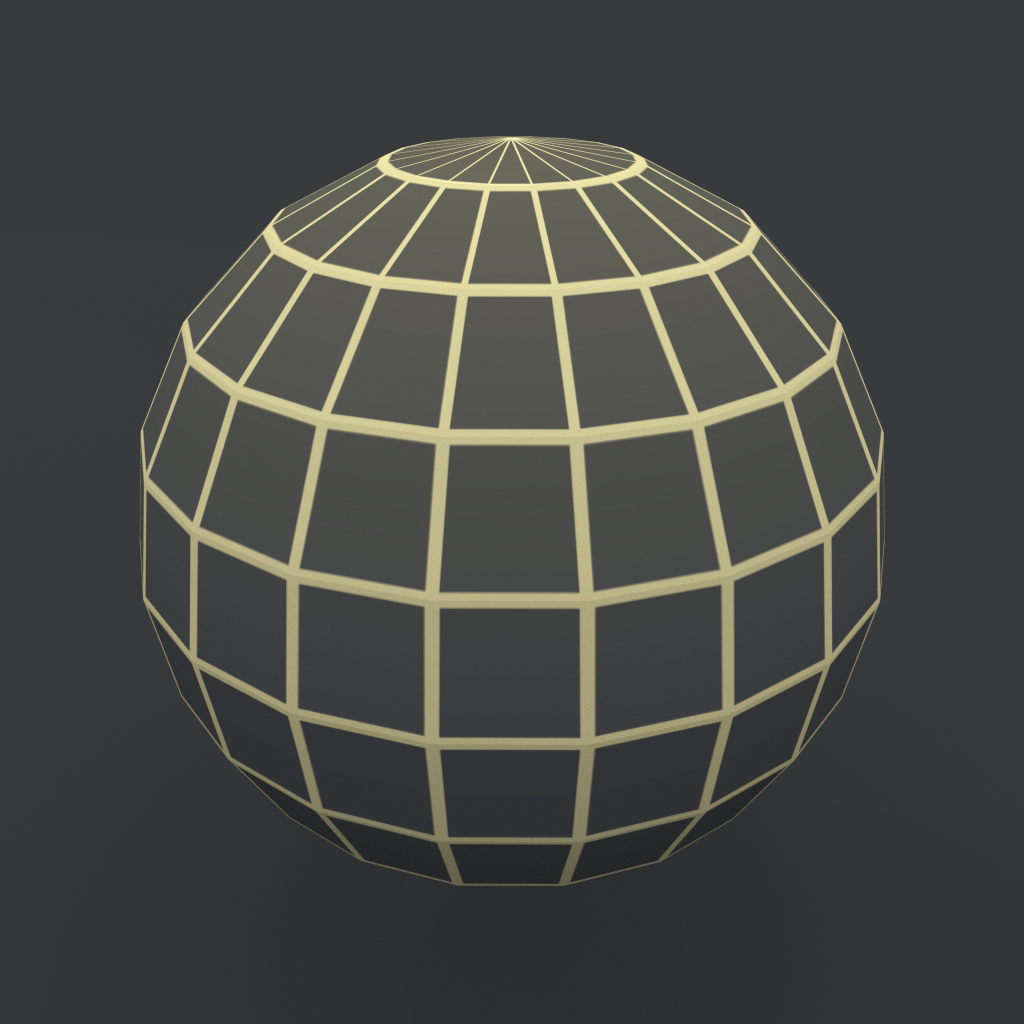
\includegraphics[width=0.95\linewidth]{figures/def3.png}
				\captionof{figure}{\emph{Sphere mapping}}
				\label{fig:def3}
			\end{minipage}
		\end{figure}
		\info[inline]{WIP}
		
		\subsection{Correlation Cartographie-Detection}
		
			\lipsum[2]
			\content[inline]{A faire}
			
		\subsection{Contrôle du robot}
		
			D'après le manuel d'utilisation du WiFibot Lab\cite{wifibot}, le robot est controllable grâce à un joystick au travers d'une application fournie dans le CD-ROM de support. Il est également possible de le contrôler au travers du protocole RS232\cite{rs232} encapsulé dans des trames \gls{udp}. L'envoi des commandes moteur s'effectue au travers de deux octets, contrôlant respectivement les roues gauches et droites. La répartition des informations dans chacun des octets est la suivante:
			\begin{center}
				\scriptsize
				\begin{tabular}[h]{|c||c||c|c|c|c|c|c|}
					\toprule
					bit0 & bit1 & bit2 & bit3 & bit4 & bit5 & bit6 & bit7 \\
					\midrule
					\specialcell{Asservissement\\ 0=OFF, 1=ON} &
					\specialcell{Sens\\ 0=Arrière, 1=Avant} &
					\multicolumn{6}{c|}{Vitesse (0 à 60)} \\
					\bottomrule
				\end{tabular}
			\end{center}
			Pour des raisons de simplification, nous n'avons utilisé que le mode asservi, le deuxième n'étant pas documenté dans la documentation officielle de notre version du robot.
			Ces commandes sont envoyées par action de l'utilisateur, soit par des touches clavier, soit en actionnant le joystick virtuel présent en \todoref.
			Les lois de contrôle sont relativement simples en raison de l'éloignement avec le sujet du stage et ne seront pas déteillées ici.
			\par
			En retour d'une commande, le robot envoie
			\begin{center}
				\scriptsize
				\begin{tabular}[h]{|c||c||c|c|c|c|c|c|}
					\toprule
					bit0 & bit1 & bit2 & bit3 & bit4 & bit5 & bit6 & bit7 \\
					\midrule
					\specialcell{Asservissement\\ 0=OFF, 1=ON} &
					\specialcell{Sens\\ 0=Arrière, 1=Avant} &
					\multicolumn{6}{c|}{Vitesse (0 à 60)} \\
					\bottomrule
				\end{tabular}
			\end{center}
			\info[inline]{WIP}
			
		\subsection{Modularité de l'IHM}
		
			\lipsum[2]
			\content[inline]{A faire}
			
	\section{Pérennisation du projet}
	
		\subsection{Manuel utilisateur et documentation}
		\label{sub:manuel}

			Le projet est destiné à être poursuivi lors de stages ultérieurs, c'est pourquoi il a été décidé de rédiger un manuel d'utilisation, autant à l'intention des développeurs que pour un utilisateur \og opérateur \fg{}. Il regroupe un manuel d'installation, un guide de résolution des problèmes, un manuel d'utilisation de l'interface homme-machine et un guide de développement, qui explique le fonctionnement du logiciel et propose des améliorations possibles.
			\par
			Ce manuel a été rédigé en Markdown \cite{markdown}, un langage de balisage léger permettant une mise en forme rapide du texte et l'inclusion d'images. Il est compilé sous la forme d'un site html statique par MkDocs\cite{mkdocs}, ce qui permet une mise en forme agréable, ainsi qu'une navigation simple et plus intuitive qu'un document \og classique \fg{}. Il est donc prêt à être hébergé sur un serveur web.
			\par
			Une documentation exhaustive de la partie \gls{ihm} a été écrite
			
		\subsection{Installation automatique}
		
			\content[inline]{A faire}
				
		\subsection{Communication interne}
		
			\content[inline]{A faire}
